% !TEX TS-program = pdflatex
% !TEX encoding = UTF-8 Unicode
\documentclass[border=0mm]{standalone}
% packages
\usepackage{tikz}
\usetikzlibrary{patterns}
\usepackage{amsmath,amssymb}
\usepackage{bm}
\usepackage{pgfplots}
\pgfplotsset{compat=1.15}
% start document
\begin{document}
% generated by ROOT (CERN)
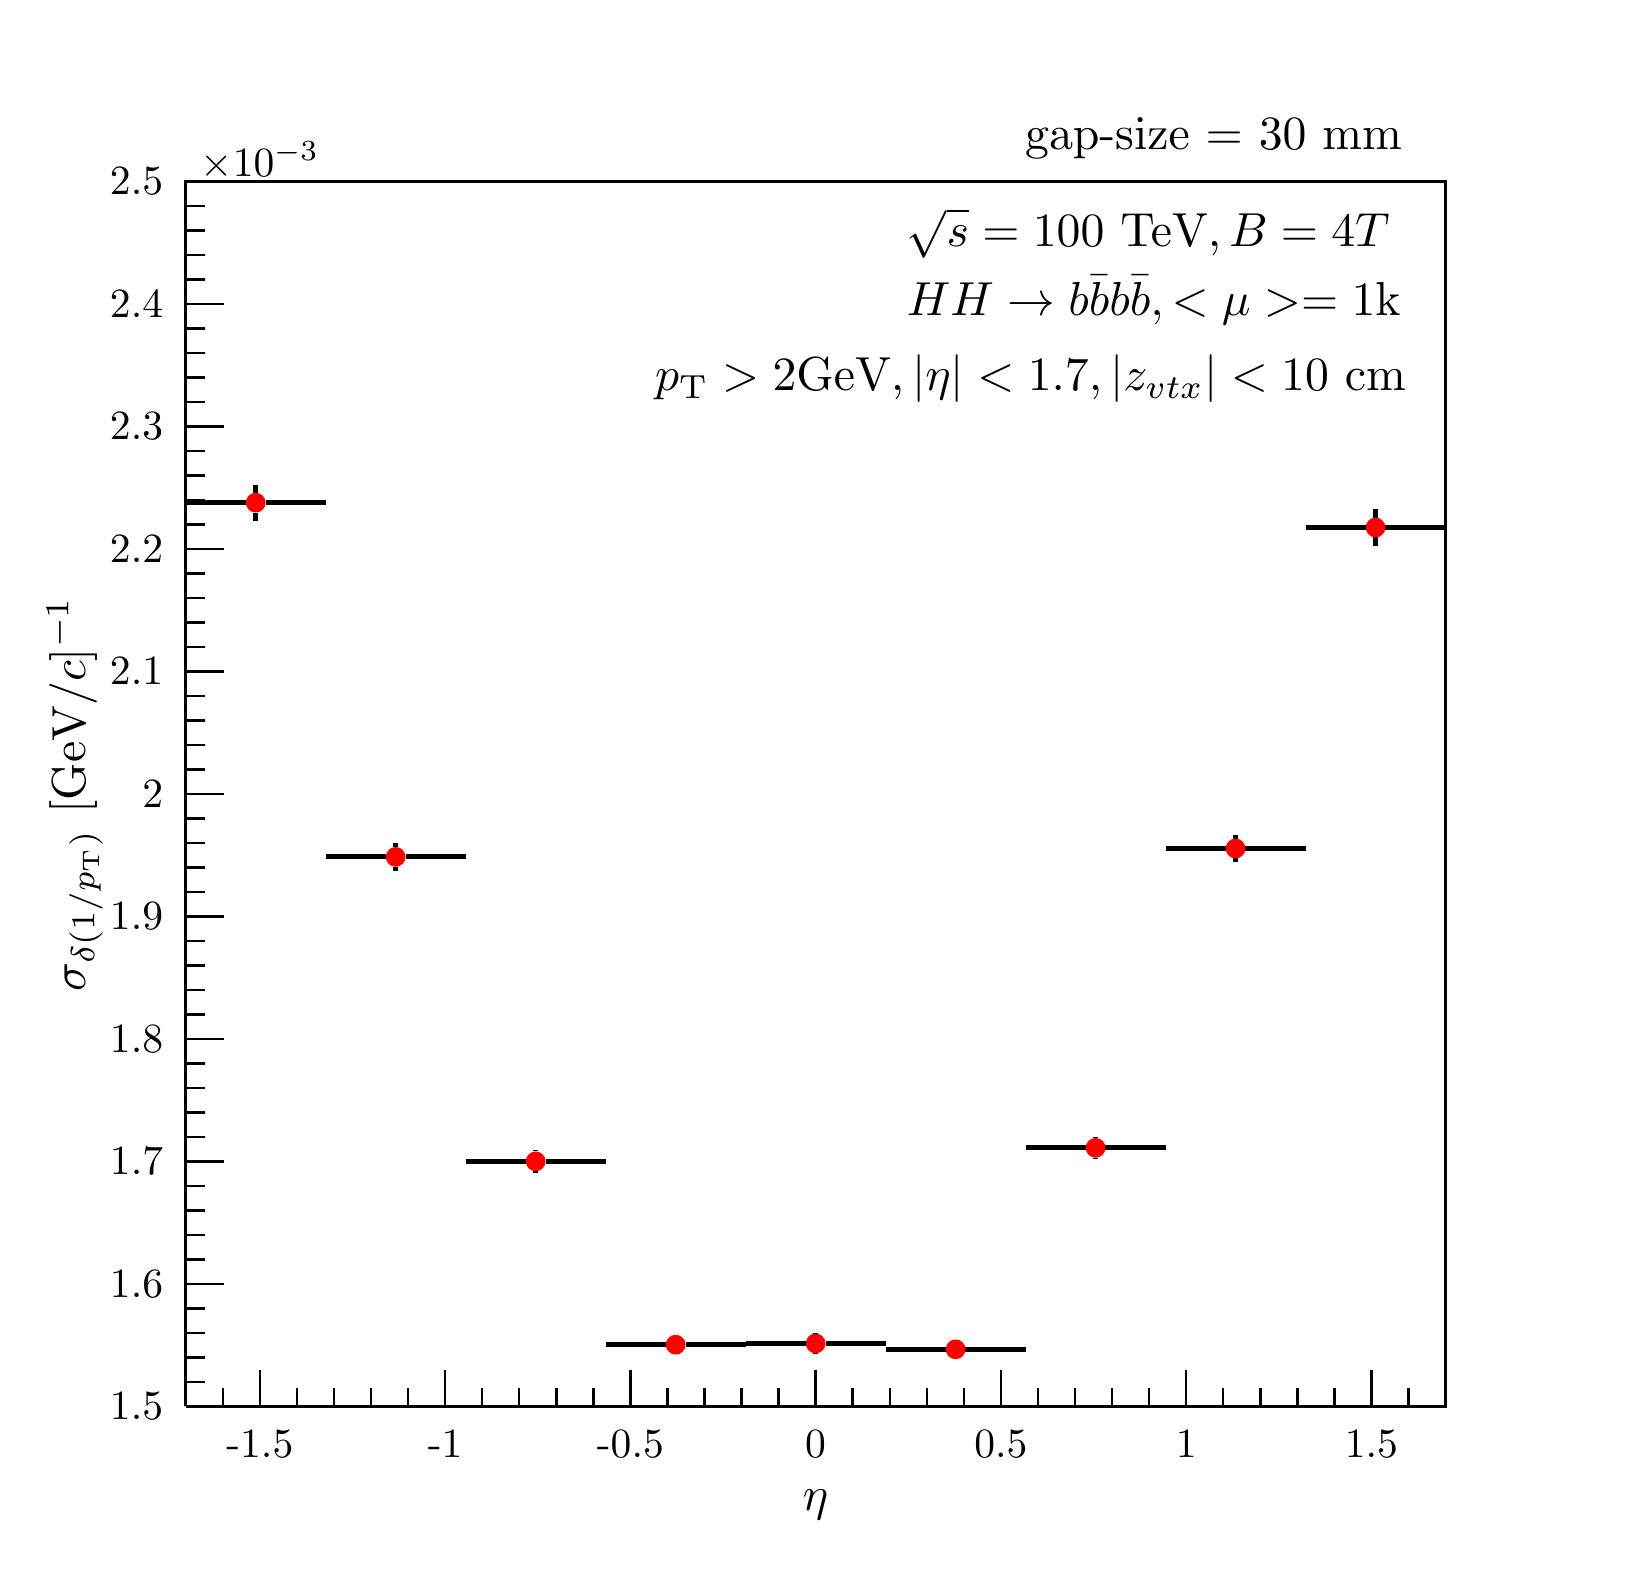
\begin{tikzpicture}
\pgfdeclareplotmark{cross} {
\pgfpathmoveto{\pgfpoint{-0.3\pgfplotmarksize}{\pgfplotmarksize}}
\pgfpathlineto{\pgfpoint{+0.3\pgfplotmarksize}{\pgfplotmarksize}}
\pgfpathlineto{\pgfpoint{+0.3\pgfplotmarksize}{0.3\pgfplotmarksize}}
\pgfpathlineto{\pgfpoint{+1\pgfplotmarksize}{0.3\pgfplotmarksize}}
\pgfpathlineto{\pgfpoint{+1\pgfplotmarksize}{-0.3\pgfplotmarksize}}
\pgfpathlineto{\pgfpoint{+0.3\pgfplotmarksize}{-0.3\pgfplotmarksize}}
\pgfpathlineto{\pgfpoint{+0.3\pgfplotmarksize}{-1.\pgfplotmarksize}}
\pgfpathlineto{\pgfpoint{-0.3\pgfplotmarksize}{-1.\pgfplotmarksize}}
\pgfpathlineto{\pgfpoint{-0.3\pgfplotmarksize}{-0.3\pgfplotmarksize}}
\pgfpathlineto{\pgfpoint{-1.\pgfplotmarksize}{-0.3\pgfplotmarksize}}
\pgfpathlineto{\pgfpoint{-1.\pgfplotmarksize}{0.3\pgfplotmarksize}}
\pgfpathlineto{\pgfpoint{-0.3\pgfplotmarksize}{0.3\pgfplotmarksize}}
\pgfpathclose
\pgfusepathqstroke
}
\pgfdeclareplotmark{cross*} {
\pgfpathmoveto{\pgfpoint{-0.3\pgfplotmarksize}{\pgfplotmarksize}}
\pgfpathlineto{\pgfpoint{+0.3\pgfplotmarksize}{\pgfplotmarksize}}
\pgfpathlineto{\pgfpoint{+0.3\pgfplotmarksize}{0.3\pgfplotmarksize}}
\pgfpathlineto{\pgfpoint{+1\pgfplotmarksize}{0.3\pgfplotmarksize}}
\pgfpathlineto{\pgfpoint{+1\pgfplotmarksize}{-0.3\pgfplotmarksize}}
\pgfpathlineto{\pgfpoint{+0.3\pgfplotmarksize}{-0.3\pgfplotmarksize}}
\pgfpathlineto{\pgfpoint{+0.3\pgfplotmarksize}{-1.\pgfplotmarksize}}
\pgfpathlineto{\pgfpoint{-0.3\pgfplotmarksize}{-1.\pgfplotmarksize}}
\pgfpathlineto{\pgfpoint{-0.3\pgfplotmarksize}{-0.3\pgfplotmarksize}}
\pgfpathlineto{\pgfpoint{-1.\pgfplotmarksize}{-0.3\pgfplotmarksize}}
\pgfpathlineto{\pgfpoint{-1.\pgfplotmarksize}{0.3\pgfplotmarksize}}
\pgfpathlineto{\pgfpoint{-0.3\pgfplotmarksize}{0.3\pgfplotmarksize}}
\pgfpathclose
\pgfusepathqfillstroke
}
\pgfdeclareplotmark{newstar} {
\pgfpathmoveto{\pgfqpoint{0pt}{\pgfplotmarksize}}
\pgfpathlineto{\pgfqpointpolar{44}{0.5\pgfplotmarksize}}
\pgfpathlineto{\pgfqpointpolar{18}{\pgfplotmarksize}}
\pgfpathlineto{\pgfqpointpolar{-20}{0.5\pgfplotmarksize}}
\pgfpathlineto{\pgfqpointpolar{-54}{\pgfplotmarksize}}
\pgfpathlineto{\pgfqpointpolar{-90}{0.5\pgfplotmarksize}}
\pgfpathlineto{\pgfqpointpolar{234}{\pgfplotmarksize}}
\pgfpathlineto{\pgfqpointpolar{198}{0.5\pgfplotmarksize}}
\pgfpathlineto{\pgfqpointpolar{162}{\pgfplotmarksize}}
\pgfpathlineto{\pgfqpointpolar{134}{0.5\pgfplotmarksize}}
\pgfpathclose
\pgfusepathqstroke
}
\pgfdeclareplotmark{newstar*} {
\pgfpathmoveto{\pgfqpoint{0pt}{\pgfplotmarksize}}
\pgfpathlineto{\pgfqpointpolar{44}{0.5\pgfplotmarksize}}
\pgfpathlineto{\pgfqpointpolar{18}{\pgfplotmarksize}}
\pgfpathlineto{\pgfqpointpolar{-20}{0.5\pgfplotmarksize}}
\pgfpathlineto{\pgfqpointpolar{-54}{\pgfplotmarksize}}
\pgfpathlineto{\pgfqpointpolar{-90}{0.5\pgfplotmarksize}}
\pgfpathlineto{\pgfqpointpolar{234}{\pgfplotmarksize}}
\pgfpathlineto{\pgfqpointpolar{198}{0.5\pgfplotmarksize}}
\pgfpathlineto{\pgfqpointpolar{162}{\pgfplotmarksize}}
\pgfpathlineto{\pgfqpointpolar{134}{0.5\pgfplotmarksize}}
\pgfpathclose
\pgfusepathqfillstroke
}
\definecolor{c}{rgb}{1,1,1};
\draw [color=c, fill=c] (0,0) rectangle (20,19.4486);
\draw [color=c, fill=c] (2,1.94486) rectangle (18,17.5038);
\definecolor{c}{rgb}{0,0,0};
\draw [c,line width=0.9] (2,1.94486) -- (2,17.5038) -- (18,17.5038) -- (18,1.94486) -- (2,1.94486);
\definecolor{c}{rgb}{1,1,1};
\draw [color=c, fill=c] (2,1.94486) rectangle (18,17.5038);
\definecolor{c}{rgb}{0,0,0};
\draw [c,line width=0.9] (2,1.94486) -- (2,17.5038) -- (18,17.5038) -- (18,1.94486) -- (2,1.94486);
\draw [c,line width=1.8] (2.88889,13.1963) -- (2.88889,13.2974);
\draw [c,line width=1.8] (2.88889,13.5481) -- (2.88889,13.6492);
\draw [c,line width=1.8] (2,13.4228) -- (2.76358,13.4228);
\draw [c,line width=1.8] (3.0142,13.4228) -- (3.77778,13.4228);
\definecolor{c}{rgb}{1,0,0};
\foreach \P in {(2.88889,13.4228)}{\draw[mark options={color=c,fill=c},mark size=3.363363pt,mark=*] plot coordinates {\P};}
\definecolor{c}{rgb}{0,0,0};
\draw [c,line width=1.8] (4.66667,8.7493) -- (4.66667,8.79863);
\draw [c,line width=1.8] (4.66667,9.04925) -- (4.66667,9.09858);
\draw [c,line width=1.8] (3.77778,8.92394) -- (4.54135,8.92394);
\draw [c,line width=1.8] (4.79198,8.92394) -- (5.55556,8.92394);
\definecolor{c}{rgb}{1,0,0};
\foreach \P in {(4.66667,8.92394)}{\draw[mark options={color=c,fill=c},mark size=3.363363pt,mark=*] plot coordinates {\P};}
\definecolor{c}{rgb}{0,0,0};
\draw [c,line width=1.8] (6.44444,4.91589) -- (6.44444,4.93253);
\draw [c,line width=1.8] (6.44444,5.18315) -- (6.44444,5.19979);
\draw [c,line width=1.8] (5.55556,5.05784) -- (6.31913,5.05784);
\draw [c,line width=1.8] (6.56976,5.05784) -- (7.33333,5.05784);
\definecolor{c}{rgb}{1,0,0};
\foreach \P in {(6.44444,5.05784)}{\draw[mark options={color=c,fill=c},mark size=3.363363pt,mark=*] plot coordinates {\P};}
\definecolor{c}{rgb}{0,0,0};
\draw [c,line width=1.8] (7.33333,2.72935) -- (8.09691,2.72935);
\draw [c,line width=1.8] (8.34754,2.72935) -- (9.11111,2.72935);
\definecolor{c}{rgb}{1,0,0};
\foreach \P in {(8.22222,2.72935)}{\draw[mark options={color=c,fill=c},mark size=3.363363pt,mark=*] plot coordinates {\P};}
\definecolor{c}{rgb}{0,0,0};
\draw [c,line width=1.8] (10,2.6099) -- (10,2.61974);
\draw [c,line width=1.8] (10,2.87036) -- (10,2.8802);
\draw [c,line width=1.8] (9.11111,2.74505) -- (9.87469,2.74505);
\draw [c,line width=1.8] (10.1253,2.74505) -- (10.8889,2.74505);
\definecolor{c}{rgb}{1,0,0};
\foreach \P in {(10,2.74505)}{\draw[mark options={color=c,fill=c},mark size=3.363363pt,mark=*] plot coordinates {\P};}
\definecolor{c}{rgb}{0,0,0};
\draw [c,line width=1.8] (10.8889,2.67081) -- (11.6525,2.67081);
\draw [c,line width=1.8] (11.9031,2.67081) -- (12.6667,2.67081);
\definecolor{c}{rgb}{1,0,0};
\foreach \P in {(11.7778,2.67081)}{\draw[mark options={color=c,fill=c},mark size=3.363363pt,mark=*] plot coordinates {\P};}
\definecolor{c}{rgb}{0,0,0};
\draw [c,line width=1.8] (13.5556,5.08528) -- (13.5556,5.10402);
\draw [c,line width=1.8] (13.5556,5.35464) -- (13.5556,5.37338);
\draw [c,line width=1.8] (12.6667,5.22933) -- (13.4302,5.22933);
\draw [c,line width=1.8] (13.6809,5.22933) -- (14.4444,5.22933);
\definecolor{c}{rgb}{1,0,0};
\foreach \P in {(13.5556,5.22933)}{\draw[mark options={color=c,fill=c},mark size=3.363363pt,mark=*] plot coordinates {\P};}
\definecolor{c}{rgb}{0,0,0};
\draw [c,line width=1.8] (15.3333,8.85572) -- (15.3333,8.90544);
\draw [c,line width=1.8] (15.3333,9.15606) -- (15.3333,9.20579);
\draw [c,line width=1.8] (14.4444,9.03075) -- (15.208,9.03075);
\draw [c,line width=1.8] (15.4586,9.03075) -- (16.2222,9.03075);
\definecolor{c}{rgb}{1,0,0};
\foreach \P in {(15.3333,9.03075)}{\draw[mark options={color=c,fill=c},mark size=3.363363pt,mark=*] plot coordinates {\P};}
\definecolor{c}{rgb}{0,0,0};
\draw [c,line width=1.8] (17.1111,12.8739) -- (17.1111,12.9825);
\draw [c,line width=1.8] (17.1111,13.2331) -- (17.1111,13.3417);
\draw [c,line width=1.8] (16.2222,13.1078) -- (16.9858,13.1078);
\draw [c,line width=1.8] (17.2364,13.1078) -- (18,13.1078);
\definecolor{c}{rgb}{1,0,0};
\foreach \P in {(17.1111,13.1078)}{\draw[mark options={color=c,fill=c},mark size=3.363363pt,mark=*] plot coordinates {\P};}
\definecolor{c}{rgb}{0,0,0};
\draw [c,line width=0.9] (2,1.94486) -- (18,1.94486);
\draw [c,line width=0.9] (2.94118,2.41163) -- (2.94118,1.94486);
\draw [c,line width=0.9] (3.41176,2.17825) -- (3.41176,1.94486);
\draw [c,line width=0.9] (3.88235,2.17825) -- (3.88235,1.94486);
\draw [c,line width=0.9] (4.35294,2.17825) -- (4.35294,1.94486);
\draw [c,line width=0.9] (4.82353,2.17825) -- (4.82353,1.94486);
\draw [c,line width=0.9] (5.29412,2.41163) -- (5.29412,1.94486);
\draw [c,line width=0.9] (5.76471,2.17825) -- (5.76471,1.94486);
\draw [c,line width=0.9] (6.23529,2.17825) -- (6.23529,1.94486);
\draw [c,line width=0.9] (6.70588,2.17825) -- (6.70588,1.94486);
\draw [c,line width=0.9] (7.17647,2.17825) -- (7.17647,1.94486);
\draw [c,line width=0.9] (7.64706,2.41163) -- (7.64706,1.94486);
\draw [c,line width=0.9] (8.11765,2.17825) -- (8.11765,1.94486);
\draw [c,line width=0.9] (8.58823,2.17825) -- (8.58823,1.94486);
\draw [c,line width=0.9] (9.05882,2.17825) -- (9.05882,1.94486);
\draw [c,line width=0.9] (9.52941,2.17825) -- (9.52941,1.94486);
\draw [c,line width=0.9] (10,2.41163) -- (10,1.94486);
\draw [c,line width=0.9] (10.4706,2.17825) -- (10.4706,1.94486);
\draw [c,line width=0.9] (10.9412,2.17825) -- (10.9412,1.94486);
\draw [c,line width=0.9] (11.4118,2.17825) -- (11.4118,1.94486);
\draw [c,line width=0.9] (11.8824,2.17825) -- (11.8824,1.94486);
\draw [c,line width=0.9] (12.3529,2.41163) -- (12.3529,1.94486);
\draw [c,line width=0.9] (12.8235,2.17825) -- (12.8235,1.94486);
\draw [c,line width=0.9] (13.2941,2.17825) -- (13.2941,1.94486);
\draw [c,line width=0.9] (13.7647,2.17825) -- (13.7647,1.94486);
\draw [c,line width=0.9] (14.2353,2.17825) -- (14.2353,1.94486);
\draw [c,line width=0.9] (14.7059,2.41163) -- (14.7059,1.94486);
\draw [c,line width=0.9] (15.1765,2.17825) -- (15.1765,1.94486);
\draw [c,line width=0.9] (15.6471,2.17825) -- (15.6471,1.94486);
\draw [c,line width=0.9] (16.1176,2.17825) -- (16.1176,1.94486);
\draw [c,line width=0.9] (16.5882,2.17825) -- (16.5882,1.94486);
\draw [c,line width=0.9] (17.0588,2.41163) -- (17.0588,1.94486);
\draw [c,line width=0.9] (2.94118,2.41163) -- (2.94118,1.94486);
\draw [c,line width=0.9] (2.47059,2.17825) -- (2.47059,1.94486);
\draw [c,line width=0.9] (2,2.17825) -- (2,1.94486);
\draw [c,line width=0.9] (17.0588,2.41163) -- (17.0588,1.94486);
\draw [c,line width=0.9] (17.5294,2.17825) -- (17.5294,1.94486);
\draw [c,line width=0.9] (18,2.17825) -- (18,1.94486);
\draw [anchor=base] (2.94118,1.30306) node[scale=1.50291, color=c, rotate=0]{-1.5};
\draw [anchor=base] (5.29412,1.30306) node[scale=1.50291, color=c, rotate=0]{-1};
\draw [anchor=base] (7.64706,1.30306) node[scale=1.50291, color=c, rotate=0]{-0.5};
\draw [anchor=base] (10,1.30306) node[scale=1.50291, color=c, rotate=0]{0};
\draw [anchor=base] (12.3529,1.30306) node[scale=1.50291, color=c, rotate=0]{0.5};
\draw [anchor=base] (14.7059,1.30306) node[scale=1.50291, color=c, rotate=0]{1};
\draw [anchor=base] (17.0588,1.30306) node[scale=1.50291, color=c, rotate=0]{1.5};
\draw (10,0.700151) node[scale=1.72557, color=c, rotate=0]{$\eta$};
\draw [c,line width=0.9] (2,1.94486) -- (2,17.5038);
\draw [c,line width=0.9] (2.48,1.94486) -- (2,1.94486);
\draw [c,line width=0.9] (2.24,2.25604) -- (2,2.25604);
\draw [c,line width=0.9] (2.24,2.56722) -- (2,2.56722);
\draw [c,line width=0.9] (2.24,2.8784) -- (2,2.8784);
\draw [c,line width=0.9] (2.24,3.18957) -- (2,3.18957);
\draw [c,line width=0.9] (2.48,3.50075) -- (2,3.50075);
\draw [c,line width=0.9] (2.24,3.81193) -- (2,3.81193);
\draw [c,line width=0.9] (2.24,4.12311) -- (2,4.12311);
\draw [c,line width=0.9] (2.24,4.43429) -- (2,4.43429);
\draw [c,line width=0.9] (2.24,4.74546) -- (2,4.74546);
\draw [c,line width=0.9] (2.48,5.05664) -- (2,5.05664);
\draw [c,line width=0.9] (2.24,5.36782) -- (2,5.36782);
\draw [c,line width=0.9] (2.24,5.679) -- (2,5.679);
\draw [c,line width=0.9] (2.24,5.99018) -- (2,5.99018);
\draw [c,line width=0.9] (2.24,6.30135) -- (2,6.30135);
\draw [c,line width=0.9] (2.48,6.61253) -- (2,6.61253);
\draw [c,line width=0.9] (2.24,6.92371) -- (2,6.92371);
\draw [c,line width=0.9] (2.24,7.23489) -- (2,7.23489);
\draw [c,line width=0.9] (2.24,7.54607) -- (2,7.54607);
\draw [c,line width=0.9] (2.24,7.85724) -- (2,7.85724);
\draw [c,line width=0.9] (2.48,8.16842) -- (2,8.16842);
\draw [c,line width=0.9] (2.24,8.4796) -- (2,8.4796);
\draw [c,line width=0.9] (2.24,8.79078) -- (2,8.79078);
\draw [c,line width=0.9] (2.24,9.10196) -- (2,9.10196);
\draw [c,line width=0.9] (2.24,9.41313) -- (2,9.41313);
\draw [c,line width=0.9] (2.48,9.72431) -- (2,9.72431);
\draw [c,line width=0.9] (2.24,10.0355) -- (2,10.0355);
\draw [c,line width=0.9] (2.24,10.3467) -- (2,10.3467);
\draw [c,line width=0.9] (2.24,10.6578) -- (2,10.6578);
\draw [c,line width=0.9] (2.24,10.969) -- (2,10.969);
\draw [c,line width=0.9] (2.48,11.2802) -- (2,11.2802);
\draw [c,line width=0.9] (2.24,11.5914) -- (2,11.5914);
\draw [c,line width=0.9] (2.24,11.9026) -- (2,11.9026);
\draw [c,line width=0.9] (2.24,12.2137) -- (2,12.2137);
\draw [c,line width=0.9] (2.24,12.5249) -- (2,12.5249);
\draw [c,line width=0.9] (2.48,12.8361) -- (2,12.8361);
\draw [c,line width=0.9] (2.24,13.1473) -- (2,13.1473);
\draw [c,line width=0.9] (2.24,13.4584) -- (2,13.4584);
\draw [c,line width=0.9] (2.24,13.7696) -- (2,13.7696);
\draw [c,line width=0.9] (2.24,14.0808) -- (2,14.0808);
\draw [c,line width=0.9] (2.48,14.392) -- (2,14.392);
\draw [c,line width=0.9] (2.24,14.7032) -- (2,14.7032);
\draw [c,line width=0.9] (2.24,15.0143) -- (2,15.0143);
\draw [c,line width=0.9] (2.24,15.3255) -- (2,15.3255);
\draw [c,line width=0.9] (2.24,15.6367) -- (2,15.6367);
\draw [c,line width=0.9] (2.48,15.9479) -- (2,15.9479);
\draw [c,line width=0.9] (2.24,16.259) -- (2,16.259);
\draw [c,line width=0.9] (2.24,16.5702) -- (2,16.5702);
\draw [c,line width=0.9] (2.24,16.8814) -- (2,16.8814);
\draw [c,line width=0.9] (2.24,17.1926) -- (2,17.1926);
\draw [c,line width=0.9] (2.48,17.5038) -- (2,17.5038);
\draw [c,line width=0.9] (2.48,17.5038) -- (2,17.5038);
\draw [anchor= east] (1.9,1.94486) node[scale=1.50291, color=c, rotate=0]{1.5};
\draw [anchor= east] (1.9,3.50075) node[scale=1.50291, color=c, rotate=0]{1.6};
\draw [anchor= east] (1.9,5.05664) node[scale=1.50291, color=c, rotate=0]{1.7};
\draw [anchor= east] (1.9,6.61253) node[scale=1.50291, color=c, rotate=0]{1.8};
\draw [anchor= east] (1.9,8.16842) node[scale=1.50291, color=c, rotate=0]{1.9};
\draw [anchor= east] (1.9,9.72431) node[scale=1.50291, color=c, rotate=0]{2};
\draw [anchor= east] (1.9,11.2802) node[scale=1.50291, color=c, rotate=0]{2.1};
\draw [anchor= east] (1.9,12.8361) node[scale=1.50291, color=c, rotate=0]{2.2};
\draw [anchor= east] (1.9,14.392) node[scale=1.50291, color=c, rotate=0]{2.3};
\draw [anchor= east] (1.9,15.9479) node[scale=1.50291, color=c, rotate=0]{2.4};
\draw [anchor= east] (1.9,17.5038) node[scale=1.50291, color=c, rotate=0]{2.5};
\draw [anchor=base west] (2,17.5718) node[scale=1.50291, color=c, rotate=0]{$\times10^{-3}$};
\draw (0.592,9.72431) node[scale=1.72557, color=c, rotate=90]{$\sigma_{\delta(1/p_{\text{T}})} ~[\text{GeV}/c]^{-1}$};
\draw [anchor=base west] (10.945,16.6748) node[scale=1.72557, color=c, rotate=0]{$\sqrt{s} = 100 ~\text{TeV}, B = 4T$};
\draw [anchor=base west] (10.945,15.7996) node[scale=1.72557, color=c, rotate=0]{$HH \rightarrow b\bar{b}b\bar{b}, <\mu> = \text{1k}$};
\draw [anchor=base east] (17.7105,14.8432) node[scale=1.72557, color=c, rotate=0]{$p_{\text{T}} > 2\text{GeV}, |\eta| < 1.7, |z_{vtx}| < 10\text{~cm}$};
\draw [anchor=base west] (12.445,17.9122) node[scale=1.72557, color=c, rotate=0]{gap-size = 30 mm};
\draw [anchor=base west] (12.445,17.5232) node[scale=1.72557, color=c, rotate=0]{ };
\end{tikzpicture}
% end document
\end{document}
